%% This is file `BeamerAnimation.tex'
%% Version: 1.0.1
%% Version date: 2018-02-19
%% 
%% Copyright (C) 2018 by Luis Paulo Laus, laus@utfpr.edu.br
%%
%% This package can be redistributed and/or modified under the terms
%% of the LaTeX Project Public License distributed from CTAN
%% archives in directory macros/latex/base/lppl.txt; either
%% version 1 of the License, or (at your option) any later version,
%% with `The Package' referring to the software `tikzlibrarysfc.code.tex' and its
%% accompanying documentation and `The Copyright Holder' referring to the
%% person Luis Paulo Laus.
%% 
%% 
%% IMPORTANT NOTICE: 
%% 
%% For error reports, comments or suggestions in case of UNCHANGED 
%% versions send mail to:
%% laus@utfpr.edu.br
%% 
%%

\documentclass{beamer}
\usepackage{tikz,units}
\usetikzlibrary{backgrounds, circuits.ee.IEC.relay}

\makeatletter
\newcommand*{\overlaynumber}{\number\beamer@slideinframe}
\makeatother

\tikzset{ % alt and visible (overlay)
  alt/.code args={<#1>#2#3}{%
    \alt<#1>{\pgfkeysalso{#2}}{\pgfkeysalso{#3}}
  },
  visible/.code args={<#1>#2}{%
    \alt<#1>{\pgfkeysalso{#2}}{}
  }
}

\colorlet{LBlue}{blue!20}
\colorlet{LRed}{red!20}

\begin{document}

\begin{frame}{Four-Step Sequencer \overlaynumber{}}
\noindent \begin{center}
\hspace*{-0.05\textwidth}\resizebox{1.1\textwidth}{!}{
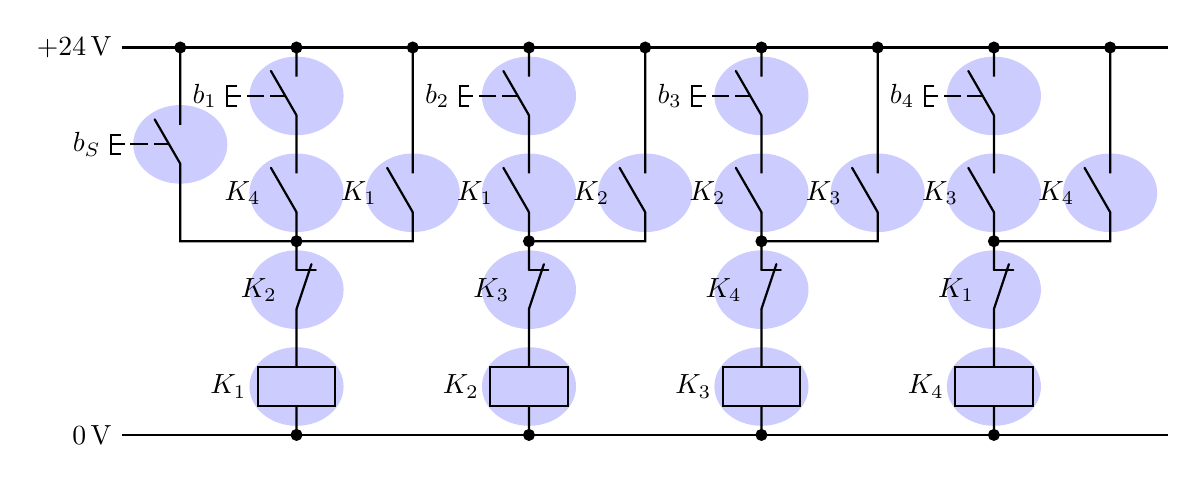
\begin{tikzpicture}[circuit ee IEC relay,thick,x=6\tikzcircuitssizeunit,y=5\tikzcircuitssizeunit]

  \draw(-1.5,0) node[left]{$\unit[0]{V}$} --+(9,0)
       (-1.5,4) node[left]{$\unit[+24]{V}$} --+(9,0);

  \draw (0,0)
    node[contact]{}
    to [relay coil={info=$K_1$,name=k11,alt={<1,2,7-17>{}{fill=LRed}}}] ++(0,1)
    to [break contact={info=$K_2$,name=k24,alt={<1-5,11-20>{}{activated}}}] ++(0,1)
    node[contact,name=N1]{}
    to [make contact={info=$K_4$,name=k43,alt={<1-13,19-20>{}{activated}}}] ++(0,1)
    to [make contact={push button={info=$b_1$},name=b1,alt={<1-16,20>{}{activated}}}] ++(0,1)
    node[contact]{};
  \draw (N1) -- ++(1,0) 
    to [make contact={info=$K_1$,name=k12,alt={<1,2,7-17>{}{activated}}}] ++(0,1) -- ++(0,1)
    node[contact]{};
  \draw (N1) -- ++(-1,0)
    to [make contact={push button={info=$b_S$},name=bs,alt={<1,4-20>{}{activated}}}] ++(0,2)
    node[contact]{};
  \draw (2,0)
    node[contact]{}
    to [relay coil={info=$K_2$,name=k21,alt={<1-5,11-20>{}{fill=LRed}}}] ++(0,1)
    to [break contact={info=$K_3$,name=k34,alt={<1-9,15-20>{}{activated}}}] ++(0,1)
    node[contact,name=N1]{}
    to [make contact={info=$K_1$,name=k13,alt={<1,2,7-17>{}{activated}}}] ++(0,1)
    to [make contact={push button={info=$b_2$},name=b2,alt={<1-4,8-20>{}{activated}}}] ++(0,1)
    node[contact]{};
  \draw (N1) -- ++(1,0)
    to [make contact={info=$K_2$,name=k22,alt={<1-5,11-20>{}{activated}}}] ++(0,1) -- ++(0,1)
    node[contact]{};
  \draw (4,0)
    node[contact]{}
    to [relay coil={info=$K_3$,name=k31,alt={<1-9,15-20>{}{fill=LRed}}}] ++(0,1)
    to [break contact={info=$K_4$,name=k44,alt={<1-13,19-20>{}{activated}}}] ++(0,1)
    node[contact,name=N1]{}
    to [make contact={info=$K_2$,name=k23,alt={<1-5,11-20>{}{activated}}}] ++(0,1)
    to [make contact={push button={info=$b_3$},name=b3,alt={<1-8,12-20>{}{activated}}}] ++(0,1)
    node[contact]{};
  \draw (N1) -- ++(1,0)
    to [make contact={info=$K_3$,name=k32,alt={<1-9,15-20>{}{activated}}}] ++(0,1) -- ++(0,1)
    node[contact]{};
  \draw (6,0) node[contact]{}
    to [relay coil={info=$K_4$,name=k41,alt={<1-13,19-20>{}{fill=LRed}}}] ++(0,1)
    to [break contact={info=$K_1$,name=k14,alt={<1,2,7-17>{}{activated}}}] ++(0,1)
    node[contact,name=N1]{}
    to [make contact={info=$K_3$,name=k33,alt={<1-9,15-20>{}{activated}}}] ++(0,1)
    to [make contact={push button={info=$b_4$},name=b4,alt={<1-12,16-20>{}{activated}}}] ++(0,1)
    node[contact]{};
  \draw (N1) -- ++(1,0)
    to [make contact={info=$K_4$,name=k42,alt={<1-13,19-20>{}{activated}}}] ++(0,1) -- ++(0,1)
    node[contact]{};
  \begin{pgfonlayer}{background}
    \visible<2-3>{
      \draw[fill=LBlue,LBlue](bs) circle (0.4);
    }
    \visible<3-6,18-20>{
      \draw[fill=LBlue,LBlue](k11) circle (0.4);
      \draw[fill=LBlue,LBlue](k12) circle (0.4);
      \draw[fill=LBlue,LBlue](k13) circle (0.4);
      \draw[fill=LBlue,LBlue](k14) circle (0.4);
    }
    \visible<5-7>{
      \draw[fill=LBlue,LBlue](b2) circle (0.4);
    }
    \visible<6-10>{
      \draw[fill=LBlue,LBlue](k21) circle (0.4);
      \draw[fill=LBlue,LBlue](k22) circle (0.4);
      \draw[fill=LBlue,LBlue](k23) circle (0.4);
      \draw[fill=LBlue,LBlue](k24) circle (0.4);
    }
    \visible<9-11>{
      \draw[fill=LBlue,LBlue](b3) circle (0.4);
    }
    \visible<10-14>{
      \draw[fill=LBlue,LBlue](k31) circle (0.4);
      \draw[fill=LBlue,LBlue](k32) circle (0.4);
      \draw[fill=LBlue,LBlue](k33) circle (0.4);
      \draw[fill=LBlue,LBlue](k34) circle (0.4);
    }
    \visible<13-15>{
      \draw[fill=LBlue,LBlue](b4) circle (0.4);
    }
    \visible<14-18>{
      \draw[fill=LBlue,LBlue](k41) circle (0.4);
      \draw[fill=LBlue,LBlue](k42) circle (0.4);
      \draw[fill=LBlue,LBlue](k43) circle (0.4);
      \draw[fill=LBlue,LBlue](k44) circle (0.4);
    }
    \visible<17-19>{
      \draw[fill=LBlue,LBlue](b1) circle (0.4);
    }
  \end{pgfonlayer}
\end{tikzpicture}}
\par\bigskip
Copyright (C) 2018 by Luis Paulo Laus, laus@utfpr.edu.br
\end{center}
\end{frame}
\end{document}